\section{Finite State Automata} \label{chp:hopcroft}

\subsection{Introduction and Motivation}
Tree compression schemes that effectively exploit repetitive structures require efficient techniques for identifying and representing such repetitions compactly. A powerful approach to this problem is to view a tree as a finite language, where each path from the root to a leaf represents a word. Such a language can be recognized by a Deterministic Finite Automaton (DFA). More specifically, since trees are inherently acyclic, they can be represented by Acyclic Deterministic Finite Automata (ADFAs).

The problem of finding and compressing identical subtrees is thus equivalent to minimizing the corresponding DFA. DFA minimization ensures that equivalent substructures are merged efficiently, leading to a more compact encoding. The minimized DFA provides a canonical representation of the repetitive structures, which can then be leveraged in our compression pipeline. This theoretical foundation enables us to identify and encode tree patterns systematically, ultimately improving the compression efficiency.

While general-purpose minimization algorithms like Hopcroft's are highly efficient for any DFA, the specific structure of ADFAs allows for even faster, linear-time algorithms. In this context, we focus on Revuz's algorithm, which is specifically designed to minimize ADFAs and is therefore particularly well-suited for compressing tree structures.

This chapter provides the necessary theoretical background on DFA minimization. We will first introduce the concepts of DFAs and their minimization, followed by a detailed look at both Hopcroft's algorithm as a general solution and Revuz's algorithm as a specialized, linear-time solution for acyclic graphs, which is central to our tree compression methodology.

\subsection{DFA Minimization}
The process of automata minimization consists of reducing the number of states in a DFA while preserving its accepted language. The minimization of DFA is crucial for a variety of applications, such as model checking, hardware design, and compilers, as it produces a more effective and compact representation of the automaton, allowing for faster processing and reduced memory usage.

The minimization of DFA is a well-studied problem in automata theory, and there are several algorithms available for this purpose. One of the most popular algorithms for DFA minimization is Hopcroft's algorithm, which was proposed by John Hopcroft in 1971 \cite{HOPCROFT1971189}. Hopcroft's algorithm is an efficient and simple algorithm that can minimize a DFA in $O(n \log n)$ time, where $n$ is the number of states in the DFA.

The algorithm enables computing equivalence classes of nodes, in particular, the Myhill-Nerode equivalence classes \cite{nerode1958linear, myhill1957finite}. The Myhill-Nerode theorem states that a language is regular if and only if it has a finite number of Myhill-Nerode equivalence classes. This theorem provides a powerful tool for determining the regularity of languages and is a cornerstone of automata theory. Let's formalize the concept of equivalence classes and the Myhill-Nerode theorem.

\begin{definition}[Myhill-Nerode Equivalence Relation]
    For a language $L \subseteq \Sigma^*$ and any strings $x,y \in \Sigma^*$, we say $x$ is equivalent to $y$ with respect to $L$ (written as $x \approx_L y$) if and only if for all strings $z \in \Sigma^*$:
    \[ xz \in L \Leftrightarrow yz \in L \]
\end{definition}
That is, strings $x$ and $y$ are equivalent if they have the same behavior with respect to the language $L$: either they both lead to acceptance or both lead to rejection when any suffix $z$ is appended.

\begin{theorem}[Myhill-Nerode theorem \cite{nerode1958linear,myhill1957finite}] \label{def:myhill-nerode}
    Let $L$ be a language over an alphabet $\Sigma$. Then $L$ is regular if and only if there exists a finite number of Myhill-Nerode equivalence classes for $L$. Specifically, the number of equivalence classes is equal to the number of states in the minimal DFA recognizing $L$.
\end{theorem}

Throughout this section let $M = (Q, \Sigma, \delta, q_0, F)$ be a DFA. For $q \in Q$ and $a \in \Sigma$, we adopt the shorthand $q.a := \delta(q,a)$. We extend $\delta$ to words by the usual recursion:
\[
\delta^{*}(q,\varepsilon) = q, \qquad
\delta^{*}(q,wa) = \delta\bigl(\delta^{*}(q,w),\, a\bigr) \quad \text{for } w \in \Sigma^{*},\ a \in \Sigma .
\]
For a word $w = w_1 w_2 \dots w_n \in \Sigma^{*}$, we then write $q.w := \delta^{*}(q,w)$ for the (unique) state reached from $q$ by reading $w$. A word $w$ is accepted by $M$ iff $\delta^{*}(q_0,w) \in F$.

Also, Let $M=(Q,\Sigma,\delta,q_0,F)$ be a DFA recognizing $L$. For states (nodes) $u,v\in Q$, we say that $u$ and $v$ are MN-equivalent iff
\[
\forall \alpha \in \Sigma^*:\ u.\alpha \in F \iff v.\alpha \in F.
\]

\begin{comment}
\subsection{Hopcroft's Minimization Algorithm}
DFA minimization is a classical and widely studied problem in Automata Theory and Formal Languages. It consists of finding the unique (up to isomorphism) finite automaton with the minimal number of states, recognizing the same regular language of a given DFA.

\begin{algorithm}
    \caption{Hopcroft's Algorithm for DFA Minimization} \label{alg:DFA_min}
    \begin{algorithmic}[1]
    \Require $M = (Q, \Sigma, \delta, q_0, F)$
    \Function{HopcroftMinimization}{$M$}
    
    \State $P \gets \{F, Q \setminus F\}$ \Comment{Initial partition}
    \State $W \gets \{F\}$ \Comment{Working set initialized with final states}
    
    \While{$W \neq \emptyset$}
        \State Remove a set $A$ from $W$
        \ForAll{$c \in \Sigma$}
            \State $X \gets \{q \in Q \mid \delta(q, c) \in A\}$ \Comment{Predecessors of $A$ via $c$}
            \ForAll{$Y \in P$ such that $X \cap Y \neq \emptyset$ and $Y \setminus X \neq \emptyset$}
                \State Replace $Y$ in $P$ with $Y_1 = X \cap Y$ and $Y_2 = Y \setminus X$
                \If{$Y \in W$}
                    \State Replace $Y$ in $W$ with $Y_1$ and $Y_2$
                \Else
                    \State Add the smaller of $Y_1$ and $Y_2$ to $W$
                \EndIf
            \EndFor
        \EndFor
    \EndWhile
    
    \State \Return the minimized DFA built from partition $P$
    \EndFunction
    \end{algorithmic}
\end{algorithm}

Algorithm \cref{alg:DFA_min} works by iteratively refining a partition of the states until no further refinement is possible, meaning all states within each set of the partition are indistinguishable. The final partition represents the equivalence classes, which correspond to the states of the minimal DFA. Here's a step-by-step explanation based on the provided pseudocode:

\begin{enumerate}
    \item \textbf{Initialization:} The algorithm starts with an initial partition $P$ containing two sets: the set of final states $F$ and the set of non-final states $Q \setminus F$. These are the coarsest sets of potentially distinguishable states. A working set $W$ is initialized, typically containing the set of final states $F$ (or the smaller of the two initial sets as an optimization). $W$ holds the sets that are used as ``splitters'' to refine the partition $P$. These sets are called ``splitters'' because they are used to partition other sets into smaller, more refined ones. A set $A \in W$ acts as a criterion to distinguish states: if for a given symbol, some states in a set $Y$ transition to a state in $A$ and others do not, then $Y$ is split.

    \item \textbf{Refinement Loop:} The algorithm iterates as long as the working set $W$ is not empty. In each iteration, a set $A$ (a ``splitter'') is removed from $W$. Then, for each input symbol $c \in \Sigma$:
        \begin{itemize}
            \item Calculate the set $X = \{q \in Q \mid \delta(q, c) \in A\}$. This is the set of all states that transition into the set $A$ upon reading symbol $c$.
            \item For each set $Y$ currently in the partition $P$, check if $Y$ needs to be split by $X$. A split is necessary if some states in $Y$ are in $X$ and some are not (i.e., $X \cap Y \neq \emptyset$ and $Y \setminus X \neq \emptyset$). This indicates that states in $Y$ are distinguishable based on whether their $c$-transition leads into $A$.
            \item If $Y$ needs to be split, replace $Y$ in the partition $P$ with two new sets: $Y_1 = X \cap Y$ (states in $Y$ that transition into $A$) and $Y_2 = Y \setminus X$ (states in $Y$ that do not transition into $A$).
            \item Update the working set $W$: If the original set $Y$ was in $W$, remove $Y$ and add both new sets $Y_1$ and $Y_2$ to $W$. If $Y$ was not in $W$, add only the smaller of the two new sets ($Y_1$ or $Y_2$) to $W$. This optimization helps maintain the algorithm's efficiency.
        \end{itemize}

    \item \textbf{Termination:} The loop continues until the working set $W$ is empty. At this point, no set in the partition $P$ can be further refined. The partition $P$ now contains the final equivalence classes of states.

    \item \textbf{Result:} The final partition $P$ defines the states of the minimized DFA. Each set in $P$ corresponds to a single state in the minimal DFA, and transitions are defined based on the original DFA's transitions between these sets.
\end{enumerate}
\end{comment}

\subsection{Revuz' Minimization Algorithm} \label{sec:revuz}
For our purpose, we will focus on a specific type of finite automaton: an acyclic deterministic finite automaton. An ADFA is a DFA where the transition graph contains no cycles. The acyclic property is key, as it simplifies the minimization process significantly. 

In this section, we will discuss an efficient algorithm for minimizing acyclic deterministic finite automata in linear time on the number of edges \cite{revuz1992minimisation}.

Let's begin by providing some definitions needed to understand the algorithm.

\begin{definition}[Height function] \label{def:height}
    For a state $s$ in an automaton, the height $h(s)$ is defined as the length of the longest path starting at $s$ and going to a final state. 

    $$h(s) = \max\{|w|:s.w \text{ is final}\}$$
\end{definition}

This height function induces a partition $\Pi_i$ of $Q$, where $\Pi_i$ denotes the set of states of height $i$.

\begin{comment}
\begin{definition}[Distinguished set]
    We say that a set $\Pi_i$ is distinguished if no pair of states in $\Pi_i$ are MN-equivalent.
\end{definition}
\end{comment}

Lets now define the canonical label of each state that will be necessary to identify MN-equivalent states. For $s\in Q$, let $l_1<\cdots<l_k$ be the symbols of the outgoing transitions defined at $s$ (listed in increasing order of $\Sigma$). With $b=\text{F}$ if $s\in F$ and $b=\text{NF}$ otherwise, we set
\[
\mathrm{l}(s) := \big(b,\, l_1,\, s.l_1,\, l_2,\, s.l_2,\, \dots,\, l_k,\, s.l_k\big).
\]

Also, the algorithm uses a function $R$ to map the labels of states to a new signature. This function is defined as follows:
\begin{definition}[Signature map $R$] \label{def:R}
Let $N[\,\cdot\,]$ be the current renaming array that assigns to each state its equivalence class identifier Myhill-Nerode.  
For a state $s$ labeled
\[
\mathrm{l}(s) \;=\; \big(b,\, l_1,\, s.l_1,\, l_2,\, s.l_2,\, \dots,\, l_k,\, s.l_k\big),
\]
where $b \in \{\text{F},\text{NF}\}$, $l_i \in \Sigma$ (listed in increasing order), and $nl_i \in Q$, define
\[
R\!\left(\mathrm{l}(s)\right) \;=\; \big(b,\, l_1,\, N[s.l_1],\, l_2,\, N[s.l_2],\, \dots,\, l_k,\, N[s.l_k]\big).
\]
\end{definition}

It is importanto to notice that, since the automaton is acyclic, every transition $s \xrightarrow{a} t$ strictly decreases the height: $h(t) < h(s)$. The main loop of \cref{alg:minimization-ADFA} processes levels in increasing order $i=0,1,\dots$, so by the time we handle a state $s\in\Pi_i$, all its targets $t$ lie in $\bigcup_{j<i}\Pi_j$ and have already been assigned a Myhill-Nerode equivalence class.

\begin{algorithm}[H]
    \caption{Revuz' Minimization Algorithm for ADFAs}
    \label{alg:minimization-ADFA}
    \begin{algorithmic}[1]
    \Require ADFA $M=(Q,\Sigma,\delta,q_0,F)$
    \Ensure Minimal DFA $M'=(\{1,\dots,n\},\Sigma,\delta',N[q_0],F')$ with $F'=\{N[q]\mid q\in F\}$ and $\delta'(N[q],a)=N[\delta(q,a)]$
    \State Calculate height $h(s)$ for every state $s$.
    \State Create partitions $\Pi_i = \{s \in Q \mid h(s) = i\}$.
    \State $N[1, |Q|] = \{1,2,\dots,|Q|\}$; \Comment{Renaming array}
    \State $n = 0$; 
    \For{$i := 0$ to $h(q_0)$} \Comment{$q_0$ is the initial state}
        \State Sort states in $\Pi_i$ based on $R(l(q)), q\in \Pi_i$.
        \State $n = n + 1$;
        \State $N[\Pi_i[1]] = n$;
        \For{$j := 2$ to $|\Pi_i|$}
            \If $R(l(\Pi_i[j])) \ne R(l(\Pi_i[j-1]))$
                \State $n = n + 1$;
            \EndIf
            \State $N[\Pi_i[j]] = n$;
        \EndFor
    \EndFor
    \end{algorithmic}
\end{algorithm}

The algorithm proceeds level by level, from $i=0$ up to the maximum height, ensuring that states at each level are correctly partitioned into Myhill-Nerode equivalence classes. For each level $i$, it groups the states in $\Pi_i$ based on their signatures computed by the function $R$ (see \cref{def:R}). As explained before, when processing level $i$, the equivalence classes for all states in lower levels ($j < i$) have already been finalized. The signature $R(l(s))$ for a state $s$ depends on its finality and the equivalence classes of its immediate successors. Therefore, two states $s, t \in \Pi_i$ have the same signature if and only if they are MN-equivalent. The algorithm assigns a unique class identifier to each group of states with the same signature.

The whole algorithm can be implemented to run in time $O(m)$ for an acyclic automaton with $m$ edges. Heights may be computed in linear time by
a bottom-up traversal. The lists of states of a given height are collected during this traversal. The signature of a state is easy to compute provided the edges starting in a state have
been sorted (by a bucket sort for instance to remain within the linear time constraint).
Sorting states by their signature again is done by a lexicographic sort \cite{berstel2010minimization}. 

\begin{example} 
    \label{ex:ADFA_minimization}
    Now we are going to see an example of reduction for a given ADFA. The ADFA is represented in figure \cref{fig:example_ADFA} and, as we can notice, it is also a valid ordered rooted tree with $n = 11$ nodes, $e = 10$ edges, and the following alphabet: $\Sigma = \{0, 1\}$. The node $a$ is the root of the tree and the initial state of the automaton, while the leaf nodes $e,g,h,i,l,m$ are final states. It is important to note that while the algorithm applies to any ADFA, our focus is on those that are also trees, as this is the specific case relevant to our work.

    \begin{figure}[H]
        \centering
        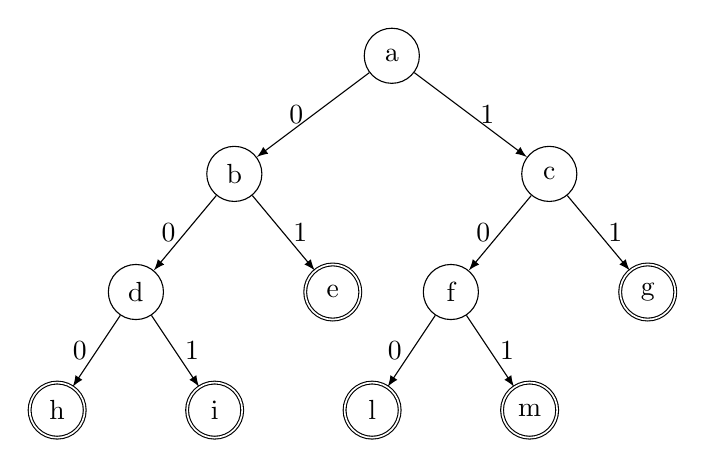
\begin{tikzpicture}[
            level distance=1.5cm,
            sibling distance=3cm,
            state/.style={circle, draw, minimum size=7mm},
            accepting/.style={circle, draw, double, minimum size=7mm},
            edge from parent/.style={draw, -latex},
            level 1/.style={sibling distance=4cm},
            level 2/.style={sibling distance=2.5cm},
            level 3/.style={sibling distance=2cm}
            ]
        
        \node[state] (a) {a}
            child {node[state] (b) {b} 
            child {node[state] (d) {d}
                child {node[accepting] (h) {h}}
                child {node[accepting] (i) {i}}
            }
            child {node[accepting] (e) {e}}
            }
            child {node[state] (c) {c}
            child {node[state] (f) {f}
                child {node[accepting] (l) {l}}
                child {node[accepting] (m) {m}}
            }
            child {node[accepting] (g) {g}}
            };
        
        % Etichette degli archi
        \path (a) -- (b) node[midway, left] {0};
        \path (a) -- (c) node[midway, right] {1};
        \path (b) -- (d) node[midway, left] {0};
        \path (b) -- (e) node[midway, right] {1};
        \path (c) -- (f) node[midway, left] {0};
        \path (c) -- (g) node[midway, right] {1};
        \path (d) -- (h) node[midway, left] {0};
        \path (d) -- (i) node[midway, right] {1};
        \path (f) -- (l) node[midway, left] {0};
        \path (f) -- (m) node[midway, right] {1};
        \end{tikzpicture}
        \caption{Example ADFA to be minimized}
        \label{fig:example_ADFA}
    \end{figure}

    Now, let's apply the minimization algorithm step by step:
    \begin{enumerate}
        \item \textbf{Height Computation:} First, we compute the height of each state. The height is the length of the longest path to a final state. The final states ($e, g, h, i, l, m$) have a height of 0. For the other states, the height is calculated as follows:
        \begin{itemize}
            \item $h(d) = 1 + \max(h(h), h(i)) = 1 + 0 = 1$
            \item $h(f) = 1 + \max(h(l), h(m)) = 1 + 0 = 1$
            \item $h(b) = 1 + \max(h(d), h(e)) = 1 + \max(1, 0) = 2$
            \item $h(c) = 1 + \max(h(f), h(g)) = 1 + \max(1, 0) = 2$
            \item $h(a) = 1 + \max(h(b), h(c)) = 1 + \max(2, 2) = 3$
        \end{itemize}
        This gives us the following partitions based on height:
        \begin{itemize}
            \item $\Pi_0 = \{e, g, h, i, l, m\}$
            \item $\Pi_1 = \{d, f\}$
            \item $\Pi_2 = \{b, c\}$
            \item $\Pi_3 = \{a\}$
        \end{itemize}

        \item \textbf{Processing $\Pi_0$:} All states in $\Pi_0$ are final and have no outgoing transitions, so they are all equivalent. We merge them into a single class, let's call it $D = \{e, g, h, i, l, m\}$. After this step, we have a new state $D$ which is final.

        \item \textbf{Processing $\Pi_1$:} Now we examine the states in $\Pi_1$: $d$ and $f$. We check their transitions:
        \begin{itemize}
            \item State $d$: $\delta(d, 0) = h \in D$ and $\delta(d, 1) = i \in D$.
            \item State $f$: $\delta(f, 0) = l \in D$ and $\delta(f, 1) = m \in D$.
        \end{itemize}
        Since both states transition to the same equivalence class ($D$) for both symbols $0$ and $1$, they are equivalent. We merge them into a new class, $C = \{d, f\}$.

        \item \textbf{Processing $\Pi_2$:} Next, we process the states in $\Pi_2$: $b$ and $c$.
        \begin{itemize}
            \item State $b$: $\delta(b, 0) = d \in C$ and $\delta(b, 1) = e \in D$.
            \item State $c$: $\delta(c, 0) = f \in C$ and $\delta(c, 1) = g \in D$.
        \end{itemize}
        Both states have transitions to class $C$ on symbol $0$ and to class $D$ on symbol $1$. Therefore, $b$ and $c$ are equivalent. We merge them into a new class, $B = \{b, c\}$.

        \item \textbf{Processing $\Pi_3$:} Finally, we process $\Pi_3$, which contains only state $a$. There is nothing to compare it with, so it forms its class, $A = \{a\}$.
    \end{enumerate}

    After applying the algorithm, we obtain the minimized ADFA represented in figure \cref{fig:example_minimized_ADFA}. Each node of the original ADFA is represented by a node in the minimized ADFA (equivalence classes). The edges represent transitions between these nodes. The root node $A$ is the initial state of the minimized ADFA, while the node $D$ is the final state.
    \begin{figure}[H]
        \centering
        \begin{tikzpicture}[->, >=stealth, node distance=3cm, on grid, auto]
            \node[state, initial, initial text=] (A) {A};
            \node[state] (B) [right=of A] {B};
            \node[state] (C) [right=of B] {C};
            \node[state, accepting] (D) [right=of C] {D};
        
            \path (A) edge [bend left] node {0} (B)
                    edge [bend right] node[below] {1} (B)
                (B) edge [bend left] node {0} (C)
                    edge [bend right] node[below] {1} (D)
                (C) edge [bend left] node {0} (D)
                    edge [bend right] node[below] {1} (D);
        \end{tikzpicture}
        \caption{Minimized ADFA}
        \label{fig:example_minimized_ADFA}
    \end{figure}      

    The equivalence classes of the nodes are listed in table \cref{tab:equivalence_classes}.
    \begin{center}
        \begin{tabular}{|c|l|}
        \hline
        \textbf{Class} & \textbf{States} \\
        \hline
        A & $a$ \\
        B & $b, c$ \\
        C & $d, f$ \\
        D & $e, g, h, i, l, m$ \\
        \hline
        \end{tabular}
        \captionof{table}{Equivalence classes of the nodes}
        \label{tab:equivalence_classes}
    \end{center}
\end{example}
